\pagestyle{fancy}
\begin{appendices}

\addtocontents{toc}{\protect\renewcommand{\protect\cftchappresnum}{\appendixname\space}}
\addtocontents{toc}{\protect\renewcommand{\protect\cftchapnumwidth}{6em}}

\thispagestyle{fancy}

%% Define your committee members. If you have less than 6, simple delete/comment the unused lines

\newcommand{\committeeMemberOne}{Gustave Flaubert}
\newcommand{\committeeMemberOneDepartment}{Romanticism}
\newcommand{\committeeMemberOneAffiliation}{France}

\newcommand{\committeeMemberTwo}{Emile Zola}
\newcommand{\committeeMemberTwoDepartment}{Naturalism}
\newcommand{\committeeMemberTwoAffiliation}{France}

\newcommand{\committeeMemberThree}{Ivan Turgenev}
\newcommand{\committeeMemberThreeDepartment}{Realism}
\newcommand{\committeeMemberThreeAffiliation}{Russia}


\newcommand{\approvalDay}{1}
\newcommand{\approvalMonth}{August}
\newcommand{\approvalYear}{2021}

%%%%%%%%%%%%%%%%%%%%%%%%%%%%%%%%%%%%%%%%%%%%%%%%%%%%%%%%%
% Do not edit these lines unless you wish to customize
% the template
%%%%%%%%%%%%%%%%%%%%%%%%%%%%%%%%%%%%%%%%%%%%%%%%%%%%%%%%%

\pagestyle{fancy}
\chapter*{\thesisTitle}
\begin{singlespacing}
\vspace{10\baselineskip}
% \vfillemplate

%Define minipages, depending on how many authors there are
\ifdefined\committeeMemberFour

Approved by:
\vspace{2\baselineskip}		%adjust the number in front of "\baselineskip" for alignment

\begin{minipage}[b]{0.4\textwidth}
	
	\committeeMemberOne\\
	\committeeMemberOneDepartment\\
	\textit{\committeeMemberOneAffiliation}\\
	
	\committeeMemberTwo\\
	\committeeMemberTwoDepartment\\
	\textit{\committeeMemberTwoAffiliation}\\
	
	\committeeMemberThree\\
	\committeeMemberThreeDepartment\\
	\textit{\committeeMemberThreeAffiliation}\\
	
	\vspace{2\baselineskip}		%adjust the number in front of "\baselineskip" for alignment
	
\end{minipage}
\hspace{0.1\textwidth}
\begin{minipage}[b]{0.4\textwidth}
	
	\committeeMemberFour\\
	\committeeMemberFourDepartment\\
	\textit{\committeeMemberFourAffiliation}\\
	
	\ifdefined\committeeMemberSix
	\committeeMemberFive\\
	\committeeMemberFiveDepartment\\
	\textit{\committeeMemberFiveAffiliation}\\
	
	\committeeMemberSix\\
	\committeeMemberSixDepartment\\
	\textit{\committeeMemberSixAffiliation}\\
	
	Date Approved: \approvalMonth{} \approvalDay, \approvalYear
	\vspace{1\baselineskip}		%adjust the number in front of "\baselineskip" for alignment
	
	\else
	
	\committeeMemberFive\\
	\committeeMemberFiveDepartment\\
	\textit{\committeeMemberFiveAffiliation}\\
		
	Date Approved: \approvalMonth{} \approvalDay, \approvalYear
	\vspace{5\baselineskip}		%adjust the number in front of "\baselineskip" for alignment
	
	\fi
	
\end{minipage}

\else

\hspace{0.4\textwidth}
\begin{minipage}[b]{0.5\textwidth}
	
	Approved by:
	\vspace{2\baselineskip}		%adjust the number in front of "\baselineskip" for alignment
	
	\committeeMemberOne\\
	\committeeMemberOneDepartment\\
	\textit{\committeeMemberOneAffiliation}\\
	
	\committeeMemberTwo\\
	\committeeMemberTwoDepartment\\
	\textit{\committeeMemberTwoAffiliation}\\
	
	\committeeMemberThree\\
	\committeeMemberThreeDepartment\\
	\textit{\committeeMemberThreeAffiliation}\\
	
	\vspace{2\baselineskip}		%adjust the number in front of "\baselineskip" for alignment
	
	Date Approved: \approvalMonth{} \approvalDay, \approvalYear
	\vspace{\baselineskip}		%adjust the number in front of "\baselineskip" for alignment
	
\end{minipage}

\fi


\end{singlespacing}

\chapter{Scaling of the Number of Matrix-Vector Multiplications $\mu$}
\label{app:muscaling}

The asymptotic behavior of runtime, discussed in Chapter~\ref{chap:scaling}, is governed by the scaling of $\mu$~\eqref{eq:mudefnition} with the dimension $d$ of the Hilbert space. The dependence $\mu(d)$ is specific to the matrix $A$ to be exponentiated (which is proportional to the Hamiltonian). This prevents a general scaling relation from being stated. I thus turn to a discussion of several concrete examples. 

I first consider the example of the transmon--cavity system, see Eq.~\eqref{eq:fockH}, where $d$ is increased via the cavity dimension $d_c$ while leaving the transmon cutoff fixed. The corresponding Hamiltonian $H_1$, written in the bare product basis, then has a constant maximum number of non-zero elements in each row. (I.e., the parameter $\sigma'$~\eqref{eq:sigmapdef} is independent of $d$.) Numerically, I find in this case that $\mu$ scales linearly with $\norm{A}_1$ \big($\mu\sim\Theta(\norm{A}_1)$\big), and this linearity holds for a wide range of $\tau$, see Fig.~\ref{fig:muscaling}(a). In this example, two ingredients lead to the scaling $\norm{A}_1\sim \Theta(d^{1/2})$: (1)~$d$ is a constant multiple of $d_c$, and (2)~the cavity ladder operators in $H_1$ which have a one-norm scaling $\Theta(d_c^{1/2})$. Thus, the overall scaling $\mu\sim \Theta(d^{1/2})$ is obtained, see Fig.~\ref{fig:muscaling}(e). In the second example, I consider the system of three coupled transmons, see Eq.~\eqref{eq:gateH}. The Hamiltonian $H_2$ is written in the harmonic oscillator basis and has a constant $\sigma'$, which leads to $\mu\sim\Theta(\norm{A}_1)$ [Fig.~\ref{fig:muscaling}(b)]. The one-norm of operator $(b^\dagger b)^2$ in $H_2$ has quadratic scaling with each transmon dimension. Since $d$ is increased by enlarging the dimensions of all three transmons simultaneously, $\norm{A}_1\sim\Theta(d^{2/3})$. This scaling results in $\mu\sim \Theta(d^{2/3})$, see Fig.~\ref{fig:muscaling}(f).

For other Hamiltonian matrices where $\sigma'$ depends on $d$, the scaling $\mu\sim\Theta(\norm{A}_1)$ may still hold. In the following, I show two concrete examples---one where linearity holds, and another where it breaks. I first consider a driven system of $N_q$ qubits with nearest-neighbor $\sigma_z$ coupling. In the rotating frame, the system is described by 
\begin{align}
\label{eq:H3}
 H_3(t)=\sum_{\nu=1}^{N_q}[a_x^{(\nu)}(t)\sigma^{(\nu)}_x+a_y^{(\nu)}(t)\sigma^{(\nu)}_y]+\sum_{\nu=1}^{N_q-1}g\sigma_z^{(\nu)}\sigma_z^{{(\nu+1)}}.
\end{align}

\begin{figure}[t]
  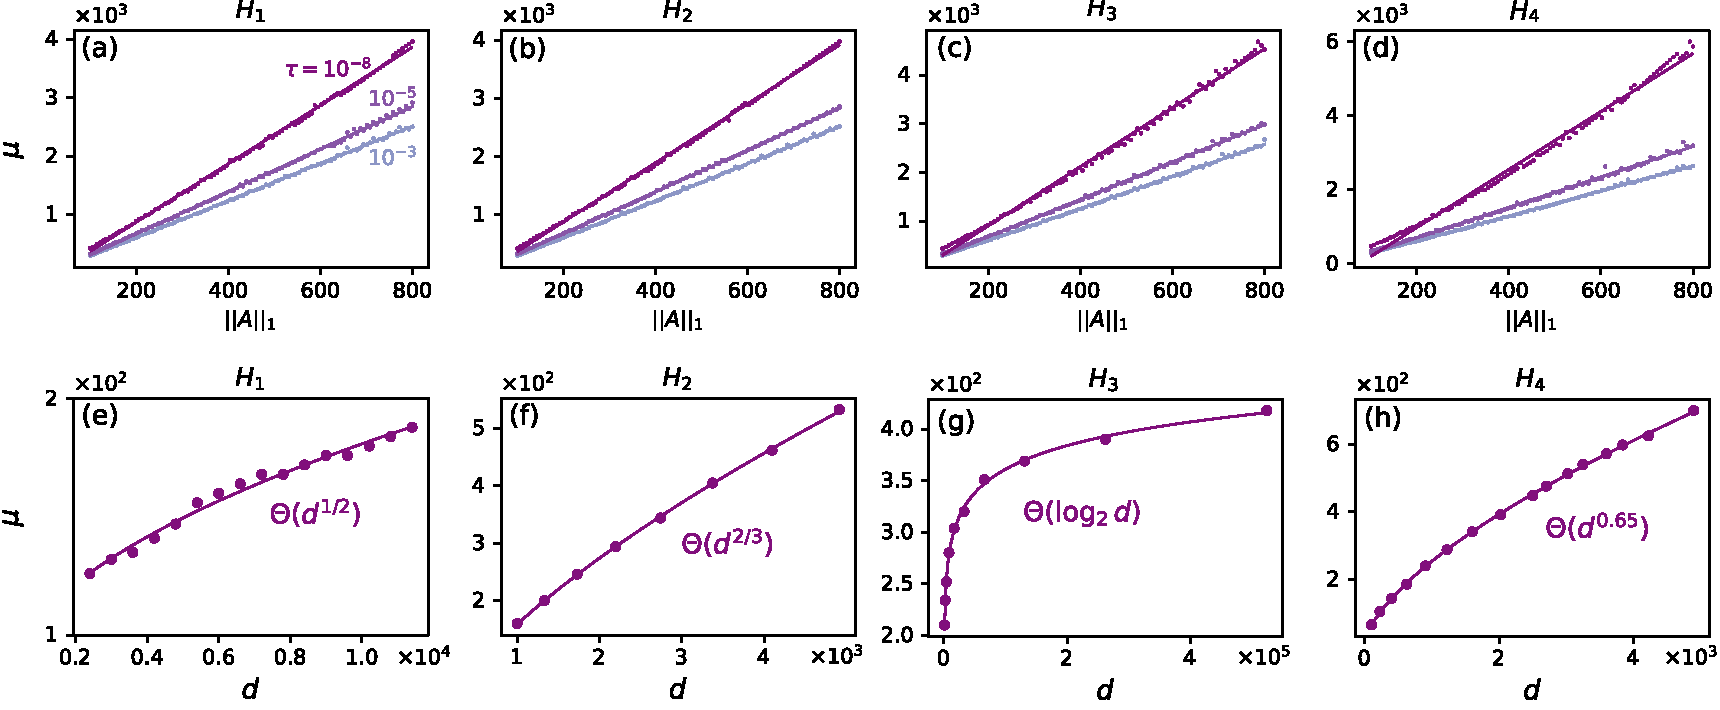
\includegraphics[width=\linewidth]{ch3_figures/uscaling.pdf}
  \caption{Scaling of $\mu$, the number of matrix-vector multiplications. (a)--(d)~The scaling of $\mu$ with $\norm{A}_1$ for Hamiltonians $H_j$, $j=1,2,3,4$, when considering several error tolerances $\tau$. (e)--(h)~The scaling of $\mu$ with dimension $d$ when considering $\tau=10^{-8}$ for each $H_j$, respectively. In all figures, dots are sampling data and solid lines are fitting curves. The parameter setup of $H_1$, $H_2$ is the same as those given in the captions of Figs.~\ref{fig:state_time} and~\ref{fig:gate}. Parameters of $H_3$ and $H_4$ are as follows: for $H_3$, $E_{Ci}/2\pi=2.5$\,GHz, $E_{Ji}/2\pi=8.9$\,GHz, $E_{Li}/2\pi=0.5$\,GHz, $g/2\pi=0.1$\,GHz, and $\phi=0.33$; for $H_4$, $a_x^{(\nu)}/2\pi=a_y^{(\nu)}/2\pi=0.5$\,GHz and $g/2\pi=0.1$\,GHz.}
  \label{fig:muscaling}
\end{figure}

Each qubit is controlled via drive fields $a_x^{(\nu)}$ and $a_y^{(\nu)}$. 
For this example, the numerical results show that the scaling $\mu\sim\Theta(\norm{A}_1)$ still holds, see Fig.~\ref{fig:muscaling}(c). Since $d$ is increased by enlarging $N_q$, $\norm{A}_1\sim\Theta(N_q)\sim\Theta(\log_2d)$. This scaling results in $\mu\sim \Theta(\log_2d)$, see Fig.~\ref{fig:muscaling}(g). For the second example, I consider two capacitively coupled fluxonium qubits with Hamiltonian
\begin{align}
\label{eq:fluxonium}    H_4(t)&=\sum_{i=1}^2 \big(4E_{Ci}n_i^2-E_{Ji}\cos(\varphi_i)+\frac{E_{Li}}{2}[\varphi_i-\phi_i(t)]^2\big) + gn_1n_2.
\end{align}
Here, $E_{Ci}$, $E_{Ji}$, $E_{Li}$ denote the charging, inductive, and Josephson energies of two fluxonium qubits, and $g$ is the interaction strength. $\varphi$ and $n$ are the phase and charge number operators, defined in the usual way. The Hamiltonian is represented in the harmonic oscillator basis. Fig.~\ref{fig:muscaling}(d) shows that the scaling of $\mu$ is superlinear with $\norm{A}_1$ for $\tau=10^{-8}$. I thus settle for a numerical determination of the scaling relation between $\mu$ and $d$ for $\tau=10^{-8}$ by increasing the dimensional cutoff for both fluxonium qubits simultaneously. The observed scaling is $\mu\sim \Theta (d^{0.65})$, see Fig.~\ref{fig:muscaling}(h). 


\chapter{Alternative Hard-Coded Gradient Scheme: Numerical Implementation and Scaling}
\label{app:matdiag}

The numerical implementation of the hard-coded gradient scheme requires evaluation of the short-time propagator and its derivative. Under certain conditions, it turns out to be advantageous to numerically evaluate the short-time propagator by employing matrix diagonalization. In this appendix, I first discuss the method to compute the propagator derivative and then analyze the scaling of HG.


\section{Evaluation of propagator derivative}
\label{sec:app_prop_deriv}

The operator $-iH\Delta t$ is anti-Hermitian, and hence can be diagonalized and exponentiated according to 
\begin{align}
\label{eq:matrix_dia}    &A=SDS^\dagger,\\
    &e^A=Se^DS^\dagger.
\end{align}
Here, $S$ is unitary and $D$ diagonal. As a result, the propagator derivative can be written as
\begin{align}
\label{eq:D1}
    \frac{d e^{A}}{d a}=Se^D\frac{dD}{da}S^\dagger+\frac{dS}{da}e^DS^\dagger+Se^D\frac{dS^\dagger}{da}.
\end{align}
Applying the inverse unitary transformation to $\frac{d e^{A}}{d a}$~\eqref{eq:D1} yields
\begin{align}
\label{eq:D3}
    S^\dagger\frac{de^A}{da}S=e^D\frac{dD}{da}+S^\dagger\frac{dS}{da}e^D+e^D\frac{dS^\dagger}{da}S.
\end{align}
Based on $\frac{dS^\dagger}{da}S+S^\dagger\frac{dS}{da}=0$, Eq.~\eqref{eq:D3} can be rewritten as 
\begin{align}
\label{eq:D4}
    S^\dagger \frac{de^A}{da}S=e^D\frac{dD}{da}+E\circ(S^\dagger\frac{dS}{da})
\end{align}
with $E_{ij}:=e^{D_{jj}}-e^{D_{ii}}$. Here, $\circ$ denotes the Hadamard product (element-wise multiplication). To obtain $dD/da$ and $dS/da$, one takes the derivative of Eq.~\eqref{eq:matrix_dia} and repeats the same steps as for Eqs.~\eqref{eq:D3} and~\eqref{eq:D4}, leading to
\begin{align}
\label{eq:D5}
    S^\dagger\frac{dA}{da}S=\frac{dD}{da}+E'\circ(S^\dagger\frac{dS}{da}),
\end{align}
where $E'_{ij}:=D_{jj}-D_{ii}$. 
Since the diagonal elements of $E'$ are zero, it follows that
\begin{align}
\label{eq:dD}
    \frac{dD}{da}=I\circ (S^\dagger\frac{dA}{da}S).
\end{align}
For off-diagonal elements of the operator in Eq.~\eqref{eq:D5}:
\begin{align}
\label{eq:dF}
    F\circ (S^\dagger\frac{dA}{da}S)+G=S^\dagger\frac{dS}{da},
\end{align}
where 
\begin{align}
    &F_{ij}:=
  \begin{cases}
    \frac{1}{D_{jj}-D_{ii}},& \text{if $D_{jj}-D_{ii} \neq 0$}.\\
    0, & \text{otherwise}.
  \end{cases}\\
\nonumber  &G_{ij}:=
  \begin{cases}
    0, & \text{if $D_{jj}-D_{ii} \neq 0$}.\\
    (S^\dagger\frac{dS}{da})_{ij}, & \text{otherwise}.
\end{cases}
\end{align}
Inserting Eqs.~\eqref{eq:dD} and~\eqref{eq:dF} into Eq.~\eqref{eq:D4} gives
\begin{align}
\label{eq:propagator_der}
    \frac{de^A}{da}=S\big((e^D+E \circ F)\circ(S^\dagger \frac{dA}{da}S)\big)S^\dagger,
\end{align}
where $E\circ G=0$ has been used. 

\section{Scaling analysis}
\label{sec:app_scaling}

The gradients of the contributions to the cost function (for the case of state transfer) are evaluated by the forward-backward propagation scheme. In this scheme, the storage required for states does not scale with the number of intermediate time steps. The matrices that must be stored are the system and control Hamiltonians as well as the dense matrices $S$, $E$, and $E'$. Thus, the total memory usage scales as $O(d^2)$. The runtime of the scheme is dominated by $O(N)$ evaluations of the propagator and its derivative. Employing matrix diagonalization for the propagator evaluation requires a runtime scaling $\sim O(d^3)$~\cite{matridiagcomppan1999complexity}. Calculation of the propagator derivative involves matrix-matrix multiplication and Hadamard product with runtime scaling $O(d^3)$ and $O(d^2)$, respectively. Thus, the overall runtime of the HG scheme scales as $O(Nd^3)$. 

The gradients of the contributions to the gate-operation cost function are evaluated in an analogous manner, resulting in the same runtime and memory scaling.

\end{appendices}
